\section{函数}
\label{sec:ru-functions}

第~\ref{sec:prelim-functions-value-ranges}节的映射可以在任意集合之间建立对应。本节集中考察输入和输出都是实数的映射，
并把三件容易混在一起的事分开：函数本身是什么，函数怎样被写出来，以及怎样由已有函数得到新函数。

\subsection{函数的定义}
\label{sec:ru-function-definition}

设$X\subseteq\mathbb R$。映射$f:X\to\mathbb R$称为实变量的实值\term{函数}（function），$X$是它的\term{定义域}（domain），$\mathbb R$是目标集。
实际取到的值组成像集$f(X)=\{f(x):x\in X\}$，有序对组成的集合$\{(x,f(x)):x\in X\}$称为函数的\term{图像}（graph）。
两个函数相等，要求定义域相同，并且在每个输入处取值相同。
所以同一个表达式配上不同的定义域，就是不同的函数：$x\mapsto x^2$在$\mathbb R$上不是单射，因为$(-1)^2=1^2$；
限制到$[0,+\infty)$上却是单射，后面正是用这种限制构造平方根。

函数可以用公式写出，如$f(x)=x^2$；也可以分段规定，如
\[
 |x|=\begin{cases}x,&x\geq0,\\-x,&x<0.\end{cases}
\]
集合$A\subseteq\mathbb R$的\term{指示函数}（indicator function）$\mathbb I_A$在$A$上取$1$、在其余位置取$0$；
$\mathbb I_{[0,+\infty)}$也写作$\mathbb I\{x\geq0\}$，称为\term{阶跃函数}（step function），它在原点从$0$跳到$1$。
函数还可以由数据表给出，只列出有限个输入处的值。
有限个值不能确定整个函数：$f(x)=x$与$g(x)=x+\sin(\pi x)$在每个整数处取值相同，因为$\sin(k\pi)=0$，
而在$x=1/2$处一个取$1/2$、一个取$3/2$。所以“与数据表一致”只限制了表中的输入，表外的值还需要别的信息。

公式中常同时出现两类字母。在$f(x)=ax+b$中，$x$是输入，取遍定义域；$a,b$在一次讨论中固定，换一组值就换了一个函数。
后一类字母称为参数，把参数取遍某个集合，就得到一族函数。下面用这个例子区分参数、整个函数、输入和函数值。

\paragraph{函数族与参数化}
\label{sec:prelim-function-families}
设想由输入预测输出：事先并不知道哪条规则最合适，通常先划定一批候选规则，再从中挑选。
这批候选规则本身是一个集合，它的元素是整个函数。具有同一定义域和目标集的一组函数组成\term{函数族}（family of functions）。
例如，形如$f(x)=ax+b$的函数称为一元\term{仿射函数}（affine function），所有这样的函数组成
\[
 \mathcal F=\{f_{a,b}:\mathbb R\to\mathbb R:\ f_{a,b}(x)=ax+b,\ (a,b)\in\mathbb R^2\}.
\]
族中的每个元素是一整个函数。取$(a,b)=(2,1)$得到函数$f_{2,1}(x)=2x+1$；再取输入$x=3$，才得到一个函数值$f_{2,1}(3)=7$。

用参数为函数族中的函数编号，称为\term{参数化}（parameterization），一般写成$\theta\mapsto f_\theta$，其中$\theta$属于参数集合$\Theta$。
这个映射的输入是参数，输出是函数；函数$f_\theta$自身的输入仍是$x$。
参数化把“在函数中挑选”改写为“在参数集合中挑选”，参数集合通常是$\mathbb R^2$这样熟悉的集合，便于后续用数值方法比较和调整。

不同参数可能表示同一个函数，所以参数与函数未必一一对应。能否由函数反过来确定参数，取决于下面的条件。
\begin{definition}[函数参数化的可识别性]
\label{def:prelim-identifiable-parameterization}
给定参数集合$\Theta$与函数族$\{f_\theta:X\to Y:\theta\in\Theta\}$。若$f_\theta=f_{\theta'}$蕴含$\theta=\theta'$，即$\theta\mapsto f_\theta$为单射，
则称这一参数化\term{可识别}（identifiable）；否则称为不可识别。
\end{definition}
这里比较的是整个定义域上的函数，而不是几个位置的函数值。仿射函数族中$b=f_{a,b}(0)$、$a=f_{a,b}(1)-f_{a,b}(0)$，
所以完整函数唯一确定$(a,b)$，这一参数化可识别。若只观察$x=0$处的函数值，则只能确定$b$，不能确定$a$。
可见“完整函数能否确定参数”与“有限个观测能否确定参数”是两个不同的问题。

\Needspace{11\baselineskip}
\begin{example}[参数不同而函数相同]
\label{ex:prelim-nonidentifiable-parameterization}
考虑参数化函数
\[
 f_{a,b}:\mathbb R\to\mathbb R,\qquad f_{a,b}(x)=abx,\qquad(a,b)\in\mathbb R^2.
\]
参数$(1,2)$与$(2,1)$不同，却对每个$x$给出相同的函数值。更一般地，只要$c\neq0$，$(ca,b/c)$与$(a,b)$就表示同一个函数。
从完整的输入输出关系可以确定乘积$ab=f_{a,b}(1)$，却不能分别确定$a$和$b$。这是参数化本身不可识别，而不是计算精度不足。
\end{example}

图~\ref{fig:vol1-add-parameter-function-value}把“由参数得到函数”和“由函数得到函数值”这两层操作分开：三组不同参数先汇入同一条完整规则，然后才在指定的$x$处求值。
\begin{figure}[!htb]
 \centering
 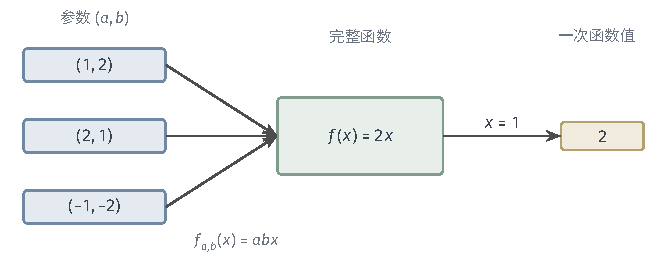
\includegraphics[width=112mm]{figures/01-mathematical-preliminaries-upper/00-shared/tikz/mathematical-language-combinatorics-analysis-optimization-comprehension-additions/parameter-function-value.pdf}
 \caption{参数化$f_{a,b}(x)=abx$中的三层对象。参数$(1,2),(2,1),(-1,-2)$的乘积均为$2$，所以它们表示同一个函数$f(x)=2x$；再指定$x=1$，才得到一次求值结果$2$。多组参数汇入同一完整函数，正是不可识别性。}
 \label{fig:vol1-add-parameter-function-value}
\end{figure}

不可识别的参数可以用第~\ref{sec:prelim-equivalence-relations}节的等价关系整理。规定$\theta\sim\theta'$当且仅当$f_\theta=f_{\theta'}$，
函数相等本身是自反、对称、传递的，所以$\sim$是参数集合上的等价关系。
每个等价类收集同一个函数的全部参数表示；在$f_{a,b}(x)=abx$中，$(a,b)$所在的等价类是满足$a'b'=ab$的全部$(a',b')$。
把每个等价类对应到它所表示的函数，得到商集$\Theta/{\sim}$到函数族的双射；参数化可识别，恰好意味着每个等价类只含一个参数。
统计模型中由有限样本推断参数时的可识别性，留到推断部分讨论。

\subsection{函数的运算}
\label{sec:ru-function-arithmetic}
\label{sec:real-function-arithmetic}

若$f,g:X\to\mathbb R$有相同的定义域，可以在每个输入处对两个函数值做实数运算：
\[
 (f\pm g)(x)=f(x)\pm g(x),\qquad (fg)(x)=f(x)g(x),\qquad (cf)(x)=cf(x),
\]
其中$c$为实常数，这些新函数的定义域仍是$X$。商只在分母不为零的输入上定义：$(f/g)(x)=f(x)/g(x)$的定义域为$\{x\in X:g(x)\neq0\}$。
例如在$\mathbb R$上取$f(x)=x$、$g(x)=x-1$，则$(f+g)(x)=2x-1$定义在整条实轴上，$(f/g)(x)=x/(x-1)$的定义域却不含$1$。
两个函数的定义域不同时，先取公共部分再运算。这些运算都作用在输出值上，与下面的复合不同。

复合把一个函数的输出送入另一个函数作为输入。设$f:X\to\mathbb R$，$g:Y\to\mathbb R$，复合$g\circ f$在$x$处的值是$g(f(x))$，
它只对满足$f(x)\in Y$的$x$有意义。例如$f(x)=1-x^2$、$g(y)=\sqrt y$（$y\geq0$），则$(g\circ f)(x)=\sqrt{1-x^2}$的定义域是$[-1,1]$，
因为只有这些$x$使$1-x^2\geq0$。复合一般不能交换次序：$(f\circ g)(y)=1-y$与$(g\circ f)(x)$是完全不同的函数。

反函数要求先有一一对应。平方函数在$\mathbb R$上不是单射，没有反函数；把定义域限制为$[0,+\infty)$后，它是$[0,+\infty)$到$[0,+\infty)$的双射，
其逆映射就是平方根$y\mapsto\sqrt y$。按第~\ref{sec:prelim-map-operations}节，反函数满足$f^{-1}(f(x))=x$与$f(f^{-1}(y))=y$。
把图像上的每个点$(x,y)$换成$(y,x)$，就得到反函数的图像，即原图像关于直线$y=x$的反射：输入与输出互换了位置。

三个记号需要分清。$f^{-1}$在反函数存在时表示反函数，$1/f$表示逐点取倒数，$f^{-1}(B)=\{x:f(x)\in B\}$表示集合的原像，后者对任何函数都有定义。
以限制在$[0,+\infty)$上的平方函数为例，$f^{-1}(4)=2$，$(1/f)(4)=1/16$；而对定义在$\mathbb R$上的平方函数，原像$f^{-1}(\{4\})=\{-2,2\}$是一个集合，它没有反函数。
